% TikZ export of an LTSpice schematic — generated by LTSpice to PDF (ASC-Parser).
% Source: 02- Resistors and wires Mirrored.asc   Skin: Default
%
% Compile on its own:   pdflatex "02- Resistors and wires Mirrored.tex"
% Or drop it into a document:
%     \usepackage{standalone}
%     ...
%     \includestandalone{02- Resistors and wires Mirrored}
%
% Lengths are in bp (PDF points), so this matches the PDF export 1:1.
\documentclass[border=0pt]{standalone}
\usepackage[T1]{fontenc}
\usepackage[utf8]{inputenc}
\usepackage{lmodern}
\usepackage{textcomp}
\usepackage{tikz}
\begin{document}
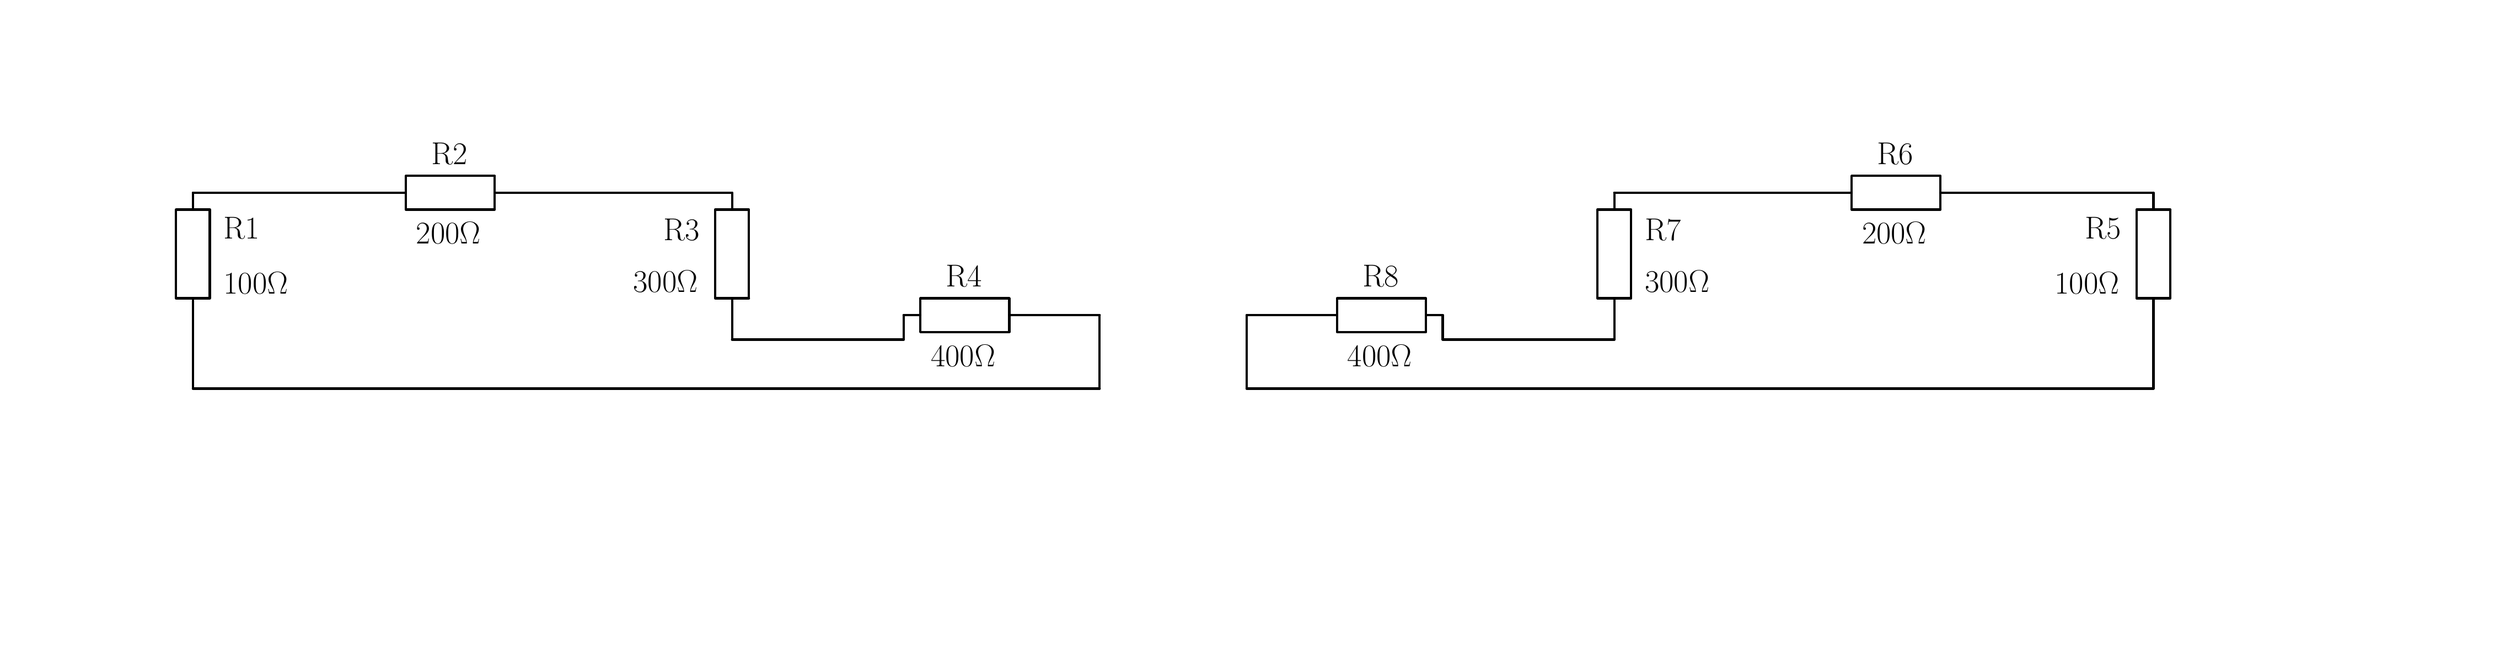
\begin{tikzpicture}[x=1bp, y=1bp, line cap=round, line join=round]
  \useasboundingbox (0,0) rectangle (1612,-412);
  \path[draw=black, line width=1.5bp] (244,-116) -- (116,-116);
  \path[draw=black, line width=1.5bp] (468,-116) -- (324,-116);
  \path[draw=black, line width=1.5bp] (1188,-116) -- (1044,-116);
  \path[draw=black, line width=1.5bp] (1396,-116) -- (1268,-116);
  \path[draw=black, line width=1.5bp] (708,-196) -- (660,-196);
  \path[draw=black, line width=1.5bp] (852,-196) -- (804,-196);
  \path[draw=black, line width=1.5bp] (468,-212) -- (468,-196);
  \path[draw=black, line width=1.5bp] (580,-212) -- (580,-196);
  \path[draw=black, line width=1.5bp] (580,-212) -- (468,-212);
  \path[draw=black, line width=1.5bp] (932,-212) -- (932,-196);
  \path[draw=black, line width=1.5bp] (1044,-212) -- (1044,-196);
  \path[draw=black, line width=1.5bp] (1044,-212) -- (932,-212);
  \path[draw=black, line width=1.5bp] (116,-244) -- (116,-196);
  \path[draw=black, line width=1.5bp] (708,-244) -- (708,-196);
  \path[draw=black, line width=1.5bp] (708,-244) -- (116,-244);
  \path[draw=black, line width=1.5bp] (804,-244) -- (804,-196);
  \path[draw=black, line width=1.5bp] (1396,-244) -- (1396,-196);
  \path[draw=black, line width=1.5bp] (1396,-244) -- (804,-244);
  \path[draw=black, line width=1.5bp] (105,-127) -- (127,-127) -- (127,-185) -- (105,-185) -- (105,-127);
  \path[draw=black, line width=1.5bp] (116,-116) -- (116,-126.9);
  \path[draw=black, line width=1.5bp] (116,-185.1) -- (116,-196);
  \node[anchor=base west, inner sep=0pt, outer sep=0pt, font=\fontsize{20bp}{24bp}\selectfont] at (136,-146) {R1};
  \node[anchor=base west, inner sep=0pt, outer sep=0pt, font=\fontsize{20bp}{24bp}\selectfont] at (136,-182) {100\textohm{}};
  \path[draw=black, line width=1.5bp] (313,-105) -- (313,-127) -- (255,-127) -- (255,-105) -- (313,-105);
  \path[draw=black, line width=1.5bp] (324,-116) -- (313.1,-116);
  \path[draw=black, line width=1.5bp] (254.9,-116) -- (244,-116);
  \node[anchor=base west, inner sep=0pt, outer sep=0pt, font=\fontsize{20bp}{24bp}\selectfont] at (271.64,-97.5) {R2};
  \node[anchor=base west, inner sep=0pt, outer sep=0pt, font=\fontsize{20bp}{24bp}\selectfont] at (261.78,-149.5) {200\textohm{}};
  \path[draw=black, line width=1.5bp] (479,-185) -- (457,-185) -- (457,-127) -- (479,-127) -- (479,-185);
  \path[draw=black, line width=1.5bp] (468,-196) -- (468,-185.1);
  \path[draw=black, line width=1.5bp] (468,-126.9) -- (468,-116);
  \node[anchor=base west, inner sep=0pt, outer sep=0pt, font=\fontsize{20bp}{24bp}\selectfont] at (423.28,-147) {R3};
  \node[anchor=base west, inner sep=0pt, outer sep=0pt, font=\fontsize{20bp}{24bp}\selectfont] at (403.56,-181) {300\textohm{}};
  \path[draw=black, line width=1.5bp] (1407,-127) -- (1385,-127) -- (1385,-185) -- (1407,-185) -- (1407,-127);
  \path[draw=black, line width=1.5bp] (1396,-116) -- (1396,-126.9);
  \path[draw=black, line width=1.5bp] (1396,-185.1) -- (1396,-196);
  \node[anchor=base west, inner sep=0pt, outer sep=0pt, font=\fontsize{20bp}{24bp}\selectfont] at (1351.28,-146) {R5};
  \node[anchor=base west, inner sep=0pt, outer sep=0pt, font=\fontsize{20bp}{24bp}\selectfont] at (1331.56,-182) {100\textohm{}};
  \path[draw=black, line width=1.5bp] (1199,-105) -- (1199,-127) -- (1257,-127) -- (1257,-105) -- (1199,-105);
  \path[draw=black, line width=1.5bp] (1188,-116) -- (1198.9,-116);
  \path[draw=black, line width=1.5bp] (1257.1,-116) -- (1268,-116);
  \node[anchor=base west, inner sep=0pt, outer sep=0pt, font=\fontsize{20bp}{24bp}\selectfont] at (1215.64,-97.5) {R6};
  \node[anchor=base west, inner sep=0pt, outer sep=0pt, font=\fontsize{20bp}{24bp}\selectfont] at (1205.78,-149.5) {200\textohm{}};
  \path[draw=black, line width=1.5bp] (1033,-185) -- (1055,-185) -- (1055,-127) -- (1033,-127) -- (1033,-185);
  \path[draw=black, line width=1.5bp] (1044,-196) -- (1044,-185.1);
  \path[draw=black, line width=1.5bp] (1044,-126.9) -- (1044,-116);
  \node[anchor=base west, inner sep=0pt, outer sep=0pt, font=\fontsize{20bp}{24bp}\selectfont] at (1064,-147) {R7};
  \node[anchor=base west, inner sep=0pt, outer sep=0pt, font=\fontsize{20bp}{24bp}\selectfont] at (1064,-181) {300\textohm{}};
  \path[draw=black, line width=1.5bp] (921,-207) -- (921,-185) -- (863,-185) -- (863,-207) -- (921,-207);
  \path[draw=black, line width=1.5bp] (932,-196) -- (921.1,-196);
  \path[draw=black, line width=1.5bp] (862.9,-196) -- (852,-196);
  \node[anchor=base west, inner sep=0pt, outer sep=0pt, font=\fontsize{20bp}{24bp}\selectfont] at (879.64,-177.5) {R8};
  \node[anchor=base west, inner sep=0pt, outer sep=0pt, font=\fontsize{20bp}{24bp}\selectfont] at (869.78,-229.5) {400\textohm{}};
  \path[draw=black, line width=1.5bp] (591,-207) -- (591,-185) -- (649,-185) -- (649,-207) -- (591,-207);
  \path[draw=black, line width=1.5bp] (580,-196) -- (590.9,-196);
  \path[draw=black, line width=1.5bp] (649.1,-196) -- (660,-196);
  \node[anchor=base west, inner sep=0pt, outer sep=0pt, font=\fontsize{20bp}{24bp}\selectfont] at (607.64,-177.5) {R4};
  \node[anchor=base west, inner sep=0pt, outer sep=0pt, font=\fontsize{20bp}{24bp}\selectfont] at (597.78,-229.5) {400\textohm{}};
\end{tikzpicture}
\end{document}
